\chapter{建立计算工作流}\label{ch:workflows}
\index{Gongzuoliu@工作流}

工作流把结构准备、电子结构求解和结果显示组织为一张可以阅读和重复运行的图。它既适合一次简单的 SCF，也适合把对称性分析、能带、态密度和结构优化串成一套计算过程。本章先介绍编辑方法，再用硅晶体和氢分子完成几条常用工作流。

如果已经完成第\ref{ch:first}章，可以从本章的硅教程继续。配套项目 \file{examples/silicon-tutorial.ks} 提供八原子硅晶胞的 SCF 与 DOS，\file{examples/silicon-band-primitive.ks} 提供二原子硅原胞的能带与对称性工作流，\file{examples/h2-tutorial.ks} 提供氢分子的 SCF 与结构优化。项目中同时保存了示例计算结果，可先查看，再重新运行。

\section{编辑工作流}

\subsection{节点怎样组织任务}
\index{Gongzuoliu jiedian@工作流节点}

画布上的一个节点代表一项任务。选择节点后，再选择 \ui{工作流 → 配置节点}，或使用节点上的齿轮，展开右侧的 \ui{配置编辑器}，打开或刷新该任务的专用 \ui{选项}。向下滚动即可查看具体参数。本章下文的“配置某节点”均采用这一操作。模块按处理阶段组织功能，任务决定节点实际做什么。标签只是画布上的名称，可以改成更容易识别的表述。

例如，一个标签为“建立硅模型”的节点可以执行 \ui{Build Molecule}；标签为“电子自洽”的节点执行 \ui{SCF}。修改标签不会自动修改任务类型。初次建立工作流时，先选择正确的任务，再决定是否需要重命名。

连线表示处理顺序。下游任务需要上游准备好的数据，能带计算需要自洽密度和路径，收敛图需要迭代历史。连线不应形成循环；几何优化中的重复求解已经由优化任务内部完成，不需要在画布上把优化节点连回自身。

\subsection{选择起始工作流}

\ui{从模板建立工作流} 中提供 SCF、Energy Band、DOS、Relaxation 和 Symmetry。模板适合学习常见任务的组合方式。打开后，选择要计算的结构并检查参数，再运行工作流。一个项目包含多个结构时，应在结构输入节点中明确选择计算对象。

从空白建立更适合定制流程。可以添加节点、调整输入输出端口、连接节点，再为每个节点指定任务。编辑画布时，可以利用缩放、适配视图、撤销和重做整理布局。清楚的布局便于查看节点之间的关系。

\begin{steps}
\item 新建空白工作流，添加第一个节点。
\item 选择节点，使用 \ui{工作流 → 配置节点} 展开配置编辑器，再设置所属模块和任务。
\item 继续添加下一个节点，并按数据处理顺序连接。
\item 逐一配置结构、物理参数和数值参数。
\item 给工作流命名并保存，然后从小规模计算开始验证。
\end{steps}

\subsection{保存项目与保存工作流的区别}

项目文件 \file{.ks} 保存结构、工作流和结果等整套内容。工作流文件 \file{.wf} 保存一张流程图及其中的任务设置，适合在不同项目之间复用计算方法。与他人分享 \file{.wf} 文件时，还需提供对应结构，并说明如何选择结构输入。

日常使用时，保存项目可保留完整计算内容。需要在其他体系上复用一套计算方法时，再将流程保存为工作流模板，并根据新体系调整结构和精度设置。


\section{选择任务}\label{sec:task-catalog}

模板覆盖常用组合，任务列表则列出可放入节点的具体工作。节点所属的\ui{模块}先确定处理阶段，\ui{任务}下拉框再选择功能。一个节点执行一种任务，任务类型在配置编辑器中选择。

\begin{longtable}{p{.28\linewidth}p{.65\linewidth}}
\caption{工作流任务及其作用。}\label{tab:task-catalog}\\
\toprule
模块与任务 & 用途和需要先准备的内容 \\
\midrule
\endfirsthead
\toprule
模块与任务 & 用途和需要先准备的内容（续） \\
\midrule
\endhead
Preprocessing & \ui{Symmetry \& K-Path}：分析晶体对称性并产生高对称路径；输入选定的晶体结构。 \\
Computation & \ui{Build Molecule}：将项目结构转为计算对象，设置泛函、赝势、截断与采样。 \\
Computation & \ui{SCF}：寻找自洽电子密度，产生基态能量、电子态和迭代历史。 \\
Computation & \ui{NSCF}：准备非自洽求解选项，供后续能带或DOS任务采用；单独运行该节点不会生成新的能带图。 \\
Computation & \ui{Geometry Optimization}：在电子计算基础上改变原子位置；需要完整的基态计算条件。 \\
Computation & \ui{TDDFT}：由基态电子态准备Casida激发态计算；参数与求解方法见本章激发态小节。 \\
Postprocessing & \ui{Band Calculation}：沿高对称路径生成k点并进行非自洽计算；需要SCF结果、NSCF选项和对称性路径。 \\
Postprocessing & \ui{Band Calculation 3D}：在选定倒空间平面上采样；需要SCF结果和NSCF选项。 \\
Visualization & \ui{Energy Curve}：把SCF能量与误差历史绘为收敛图。 \\
Visualization & \ui{Band Structure}：绘制路径能带，读取Band Calculation结果。 \\
Visualization & \ui{Band Structure 3D}：绘制采样平面上的能量曲面，读取Band Calculation 3D结果。 \\
Visualization & \ui{DOS}：采用NSCF网格计算并显示总态密度。 \\
Visualization & \ui{Brillouin Zone 2D}：显示二维布里渊区及路径，读取对称性分析结果。 \\
Visualization & \ui{Brillouin Zone 3D}：显示三维布里渊区及路径，读取对称性分析结果。 \\
\bottomrule
\end{longtable}

表中的任务名与列表中的英文一致。前处理回答“模型和路径怎样定义”，计算任务准备电子结构，后处理在所得电子态上继续采样，可视化把已有数据变成图。DOS还在自身任务中进行网格采样，因此不能只按模块名称推断它是否需要数值计算。

\section{为节点添加端口}

节点上方的端口接受前序连线，下方的端口连接后续节点。\ui{0-0 节点}没有上下端口，\ui{0-1 节点}只有下端口，\ui{1-0 节点}只有上端口，\ui{1-1 节点}上下各有一个。它们描述的是画布连接形式，不是四种不同求解器。

\begin{steps}
\item 激活一张空白工作流，打开\ui{工作流 → 添加节点}的下拉菜单，先添加一个\ui{0-1 节点}。
\item 将它配置为\ui{Computation Module → Build Molecule}，选择已经导入的结构。
\item 再添加两个\ui{1-1 节点}，分别配置为\ui{SCF}和\ui{Energy Curve}，后者属于\ui{Visualization Module}。
\item 从前一个节点下方的端口拖动到后一个节点上方端口，依次连好三个节点。
\item 若选错端口形式，选中节点后用\ui{编辑节点}中的添加或移除上、下端口调整；删除仍在使用的端口前，先核对连线。
\item 用\ui{放大}、\ui{缩小}和\ui{适配视图}看清整个流程，再保存项目。
\end{steps}

完成连线后，检查每个节点的任务与参数，然后运行SCF工作流。撤销和重做可以恢复画布编辑；保存\file{.wf}便于下次在另一个项目导入同一流程。

\section{读懂节点的通用设置}

配置节点时，\ui{通用}用于标签、模块和任务；\ui{选项}与\ui{高级选项}才是该任务的计算参数。更换任务会换成另一组参数，不会自动把前一种任务的设置逐项转换过去。先选择任务，再填写对应参数。

\ui{输入}、\ui{资源}和\ui{输出}也在编辑器中显示。\ui{资源}中的并行环境、进程数与线程数会参与实际执行；输入访问、输出保存与传递的勾选项，以及资源中的\ui{时间限制}，不执行结果筛选或自动中止。运行结果可在\ui{Results}中查看，保存项目即可保留。

\section{为计算节点分配资源}\label{sec:node-resources}
\index{Bingxing jisuan@并行计算}

\subsection{先区分节点顺序与节点内部的并行}

工作流按连线确定的先后关系依次执行节点。把画布画成两条分支，并不会让两条分支同时计算。节点内部的并行则把一项任务中的部分数值工作分给多个计算进程，例如在非自洽计算中分配不同的k点。两者的设置与作用各不相同。

配置入口位于当前节点的\ui{资源}面板。先选节点，再点击\ui{工作流 → 配置节点}，展开\ui{资源}，便可查看这个任务允许采用的执行方式。可选方式随任务与\ui{DiagMethod}所选的对角化方法改变。

\begin{table}[!htb]
\centering
\caption{节点资源字段的含义。}
\label{tab:node-resource-fields}
\begin{tabularx}{\linewidth}{lX}
\toprule
字段 & 如何理解与填写 \\
\midrule
并行环境 & 选择\ui{串行}、\ui{并行（进程池）}、\ui{GPU（对角化）}，或在支持的后续任务中\ui{继承 NSCF 配置}。实际可选项由当前任务决定。\\
最大进程数 & 正整数，默认2；限制进程池的Worker数。仅在进程池模式下可编辑。\\
线程/进程 & 正整数，默认1；限制每个计算进程的CPU计算线程数。可在进程池或GPU模式下编辑。\\
时间限制 & 可见No Limit、30 minutes、1 hour、2 hours；此字段不触发自动停止。\\
\bottomrule
\end{tabularx}
\end{table}

一个Worker是参与运算的计算进程。假设设置最大进程数2、线程/进程1，意思是最多使用两个Worker，每个Worker最多使用一个CPU计算线程。主应用本身还需要运行界面和安排任务，因此这两个数不能直接当作操作系统中全部进程与线程的总数。增加Worker也会增加内存占用，小型练习未必更快。

\ui{串行}表示这一节点不启用进程池或GPU计算，并不强制CPU只使用一个核心；数值库仍可能使用自身的CPU线程。\ui{线程/进程}也不是线程型并行池的开关。节点进程池使用进程型Worker。

\subsection{查看当前任务支持的方式}

\begin{table}[!htb]
\centering
\caption{常用任务的资源选择。}
\label{tab:node-resource-support}
\begin{tabularx}{\linewidth}{p{.29\linewidth}X}
\toprule
任务 & 当前可以选择的方式 \\
\midrule
SCF & 串行；采用受支持的对角化方法时可选GPU。此节点不提供进程池并行。\\
NSCF & 串行；关闭HT插值时可用进程池，并在方法受支持时可选GPU。这里保存的资源可由后续能带与DOS任务继承。\\
Band Calculation、DOS & 串行、继承NSCF、进程池，以及受方法支持的GPU。启用HT插值时不提供进程池或GPU。\\
Band Calculation 3D & 串行、继承NSCF、进程池，以及受方法支持的GPU；此任务直接进行NSCF采样，不采用HT插值。\\
其余任务 & 当前资源列表为串行，包括结构建立、对称性分析、几何优化、TDDFT及一般绘图任务。\\
\bottomrule
\end{tabularx}
\end{table}

GPU选项适用于\texttt{lobpcg}、\texttt{davidson}、\texttt{davidson2}和\texttt{davpcg}这些对角化方法。SCF默认的\texttt{davidson\_qe}不在此列，因此初次打开SCF资源面板时可能只见串行。GPU加速用于受支持的对角化步骤，其他计算与绘图仍按各自的执行方式运行。GPU模式中的\ui{线程/进程}限制CPU端计算线程，GPU内核线程由设备管理。

能带和DOS采用前序NSCF节点的对角化选项，因此判断其资源选择时，也要检查NSCF的\ui{DiagMethod}与\ui{Use HT}。修改任务或方法后，原先不再适用的资源选择可能恢复为串行；运行前重新打开资源面板核对一次。后续节点采用\ui{继承 NSCF 配置}时，显示继承的进程与线程数量，两个数值框不可直接编辑。需要改变它们，应返回NSCF，或在后续节点选择自己的执行方式。

一张工作流中若放置多个NSCF节点，后续采样采用执行顺序中最近一次经过的NSCF配置；它不按画布上的距离选择，也不分别为每条分支保存一套独立配置。需要比较不同资源或求解条件时，可先各保存一张工作流，使每次继承的来源清楚。

\subsection{练习：给硅\headinglatin{DOS}设置两个\headinglatin{Worker}}

这项练习沿用本章的硅DOS工作流，不改变结构、截断能、k点网格、能量范围或步长。先完成串行参考运行，再比较另一种执行方式，较容易判断差别来自计算条件还是运行环境。

\begin{steps}
\item 打开硅DOS工作流，选择\ui{NSCF}节点，点击\ui{配置节点}。
\item 在\ui{选项}中保持\ui{DiagMethod}为\texttt{lobpcg}，并使\ui{Use HT}保持关闭。
\item 展开\ui{资源}，把\ui{并行环境}改为\ui{并行（进程池）}；填写\ui{最大进程数}为2、\ui{线程/进程}为1。
\item 选择\ui{DOS}节点，查看其资源面板，选择\ui{继承 NSCF 配置}，核对显示的数量为2和1。
\item 保存项目。在执行环境提供相应并行能力后运行整张工作流，查看日志中的k点计算信息，再检查新产生的DOS结果。
\item 记录本次资源设置和用时。如需恢复串行比较，将NSCF改为\ui{串行}，再核对DOS仍然继承该设置。
\end{steps}

NSCF节点主要准备求解选项，不在这一节点上完成整条能带或DOS采样。真正使用进程池的是后续进行非自洽求解的任务。k点数大于1时，受支持的k点循环才会分给多个Worker；只在单一k点上计算，不能据此期待获得相同的并行收益。选择\ui{串行}会关闭本次节点的进程池计算路径，但保留已有并行池。

资源设置不改变所要求解的物理模型。比较结果时，仍须核对收敛、采样及能量参照；不同执行方式可能产生数值末位的差别。第一次建立并行池所需的时间也应与实际求解时间分开理解。


\begin{figure}[!htb]
\centering
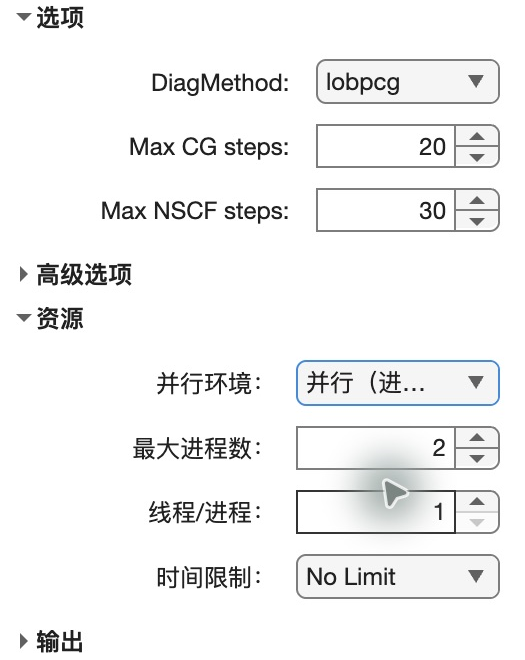
\includegraphics[width=66mm]{publication-assets/revision-nscf-process-resources.png}
\caption{NSCF节点的资源设置局部：选择进程池，最多两个Worker，每个Worker一个CPU计算线程。}
\label{fig:nscf-resources-live}
\end{figure}

\begin{figure}[!htb]
\centering
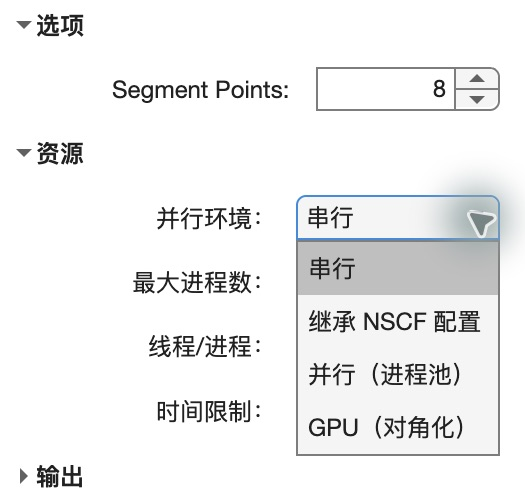
\includegraphics[width=70mm]{publication-assets/revision-band-resource-options.png}
\caption{Band Calculation节点提供继承NSCF配置的选项，也可另选自己的执行方式。}
\label{fig:band-inherit-live}
\end{figure}

\FloatBarrier
\subsection{处理资源不可用的提示}

下拉框中的一种方式表示任务支持这种计算路径，运行时还要检查执行机器的环境。进程池需要可用的Parallel Computing Toolbox与进程型池配置；GPU需要可用且受支持的GPU及相应计算组件。浏览器中的画面在个人电脑上显示，计算资源却由运行应用的服务器提供。在线版首页的\ui{并行}按钮禁用，不等于节点资源面板中的并行一律不可用；能否执行，应看节点选择及服务器实际提供的环境。

如果还没有池，应用会尝试按节点的\ui{最大进程数}建立本地进程池。请求的进程数超过本地配置允许的Worker数时，会报告数量超限，不会自行改成更大的池。如果已有池，程序会检查池的类型、Worker数与每个Worker的CPU线程数；线程型池、超过节点上限的池，或线程数超过限制的池，都会产生冲突提示。已有且满足限制的较小池可以继续使用，\ui{最大进程数}不保证每次都新建恰好这么多Worker。

尚未配置并行环境时，可先把节点改为串行，完成小型练习，再核对执行环境。完整MATLAB\regmark{}用户若自行建立过池，可先关闭不相容的池，再按节点设置运行；应用保留用户已有池的配置。由当前节点自行建立的临时池，会在该任务结束或退出时释放。

\subsection{把节点设置带到远程环境}

节点资源决定任务怎样使用计算资源；第\ref{ch:remote}章的远程配置决定任务提交到哪里。这两项可以同时使用，但填写两个Worker不会自动把任务送到集群，也不会改变节点的先后顺序。

远程提交会携带节点资源设置。远端作业已经运行在Worker中时，不能再依靠节点临时建立一个嵌套进程池；需在提交作业时预留满足节点限制的进程池，并使远端Worker的线程数相容。例如节点限制为最多2个Worker、每个1线程，远端已有4个Worker的池就不符合这个上限。集群配置中的Worker数量、PoolSize和节点中的限制应一起检查。

在线版状态栏的CPU与内存读数用于观察当前会话，不是资源申请按钮。保存项目时一并保存节点设置；记录远程计算时，还应保留所选集群及提交条件，以便下次在同一环境复现。


\section{硅晶体：建立第一个周期计算}

\subsection{准备八原子硅晶胞}

硅是理解周期计算和半导体能带的良好例子。本教程使用包含八个硅原子的立方晶胞，晶格常数为 $5.4437023729$ Å，结构保存在 \file{examples/silicon.cif}。它与软件中其他名称相近的硅文件可能有不同晶格常数，进行数值比较时请使用本书提供的文件。

自行建立项目时，按以下步骤操作。若已打开\file{silicon-tutorial.ks}，可直接选择其中的硅SCF工作流，转到下一节核对条件。

\begin{steps}
\item 保存并关闭已有项目，返回空项目。
\item 导入 \file{silicon.cif}，在三维视图中确认模型有八个独立硅位点和立方晶胞。
\item 首次保存为 \file{silicon-learning.ks}。
\item 适当显示晶胞边界，旋转模型，观察原子的空间排列。
\item 打开 SCF 模板，并把结构输入指向本例硅晶体。
\end{steps}

周期晶体的查看器可能显示跨晶胞边界的连键或相邻周期像。显示中出现重复原子并不总意味着文件里多导入了一组原子。判断原子数量应结合结构信息，判断周期连接则结合晶胞边界。


\subsection{设置 \headinglatin{SCF} 条件}

硅工作流使用 \ui{Crystal} 类型。与氢分子的主要区别是周期采样和空态数：本例以 $2\times2\times2$ 网格建立自洽密度，并增加四条空能带，以观察低能未占据态。能带一节将另用二原子标准原胞，DOS 继续使用本节的八原子晶胞。

\begin{table}[htbp]
\centering
\caption{硅教程的 SCF 设置}
\begin{tabularx}{\linewidth}{lX}
\toprule
位置 & 设置\\
\midrule
Build Molecule / Type & Crystal\\
结构 & 只选择本书的 silicon 结构\\
Functional / Pseudopotential & PBE / default\\
Ecut (Hartree) & 20\\
Smearing / Temperature & fermi-dirac / 0 K\\
Nspin & 1\\
\mbox{\ui{Autokpts}} & \mbox{\texttt{[2 2 2 0 0 0]}}\\
Extra bands & 4\\
SCF / DiagMethod & davidson\_qe\\
SCF / Max SCF steps & 100\\
\bottomrule
\end{tabularx}
\end{table}

这组参数使计算量保持较小，便于完整练习周期计算。需要提高总能量、带隙或DOS的精度时，可按第\ref{ch:theory}章的方法检查截断能和k点密度的收敛。

\subsection{运行和检查}

选择硅的 SCF 工作流并运行。确认日志中的结构名称和加载的硅赝势与本例一致，等待电子自洽完成，随后查看能量曲线。本例经过七次 SCF 迭代完成计算，总能量约为 $-31.1058309605$ Ha，最后相对密度误差约为 $7.35\times10^{-9}$。

这个总能量对应八原子晶胞。若要与原胞、超胞或每原子能量比较，先统一归一化方式；八原子晶胞的总能量不能直接与二原子原胞的总能量并列判断高低。

\section{硅晶体：沿高对称路径计算能带}
\index{Nengdai@能带}

\subsection{能带工作流要完成什么}

一幅能带图展示不同电子能量随波矢的变化。它沿若干有代表性的高对称方向绘制，因此比直接罗列所有 k 点的本征值更便于阅读。完整流程包括建立结构、分析对称性、完成电子自洽、设置非自洽求解、沿路径计算和绘图。

本节改用二原子标准硅原胞，文件为 \file{examples/silicon_primitive.cif}，也可以直接打开 \file{examples/silicon-band-primitive.ks}。原胞的三个等长晶格向量互成 $60^\circ$，长度约 $3.84928$ Å；其周期结构与前面的八原子常规胞相同。推荐高对称路径按标准原胞的倒格坐标给出，使用相应原胞可以使路径坐标与计算晶格保持一致。从 \ui{Energy Band} 模板开始。典型任务关系为 \ui{Build Molecule} 提供结构，\ui{Symmetry \& K-Path} 给出路径，\ui{SCF} 给出密度，\ui{NSCF} 给出后续求解选项，\ui{Band Calculation} 结合路径与密度完成计算，最后由 \ui{Band Structure} 显示结果。

在画布上，对称性分析和 SCF 可以表现为不同分支。检查重点是能带计算之前已经具备两类信息，而不是要求所有节点一定排成单独的一列。使用模板时，保留原有依赖关系，再调整版面位置即可。


\subsection{配置对称性和路径}
\index{Duichenxing@对称性}

首先在 \ui{Build Molecule} 中只选择二原子 \file{silicon_primitive} 结构。保持 Crystal、PBE、default、20 Ha、Nspin = 1、0 K，并使用 \mbox{\texttt{[2 2 2 0 0 0]}} 自洽网格和额外 4 条能带。原胞的整数网格与常规胞的同名整数网格对应不同采样密度，两者的每原子能量不能据此直接作精度比较。随后选择 \ui{Symmetry \& K-Path}，保持本例默认的晶格比较阈值 $10^{-7}$、对称性精度 $10^{-5}$、角度容差 $-1$。分析得到的空间群应与结构的实际几何一致。

推荐路径根据当前晶体决定。不同晶胞、轻微畸变或对称性设置可能得到不同路径。对于这个教程，先接受软件给出的推荐，再在结果中核对高对称点标签。将来研究应变或缺陷时，路径变化本身也可能反映结构对称性的改变。

\subsection{选择非自洽求解选项}

NSCF节点的\ui{DiagMethod}选择电子态求解方法。\ui{Max CG steps}与\ui{Max NSCF steps}控制两层迭代的步数，而不是路径上k点的数量；路径采样点数在后续Band Calculation节点填写。增加路径分辨率时，调整Band Calculation的采样点数。

\begin{table}[htbp]
\centering
\caption{NSCF节点的基础选项。}
\begin{tabularx}{\linewidth}{lX}
\toprule
字段 & 默认值和使用含义 \\
\midrule
DiagMethod & lobpcg；其他示例采用不同方法时，按对应参数表填写。 \\
Max CG steps & 20，LOBPCG的内部迭代步数上限。 \\
Max NSCF steps & 30，非自洽求解的外层迭代上限。 \\
Use GACE & 默认不勾选，属于专门的交换处理设置。 \\
Use HT & 默认不勾选，使用Hamiltonian transformation插值时才涉及。 \\
\bottomrule
\end{tabularx}
\end{table}

HT插值需要基态波函数与本征值等完整输入。本书PBE路径能带与DOS例均保持GACE、HT关闭，采用直接的非自洽采样。完整MATLAB\regmark{}中的高级计算应同时保存这些输入。


\subsection{设置非自洽和路径采样}

\begin{steps}
\item 在 \ui{SCF} 中保留 davidson\_qe 和最大 100 步。
\item 在 \ui{NSCF} 中保持默认 lobpcg、Max CG steps 为 20、Max NSCF steps 为 30。
\item 保持 \ui{Use GACE} 与 \ui{Use HT} 不选中。
\item 选择 \ui{Band Calculation}，将 \mbox{\ui{Segment Points}} 设为 \texttt{8}。
\item 检查最后的 \ui{Band Structure} 节点，然后保存项目。
\end{steps}

八点采样便于快速看到图形轮廓，包含每一段的两个端点。需要更平滑的曲线时，可以改为 $20$ 或更多点再运行。增加路径点数主要增加后续求解工作量，不会替代前面 SCF 网格的收敛检查。

\subsection{运行并阅读图形}

使这张能带工作流成为当前文档并运行。SCF完成后，程序继续沿路径计算。等待能带绘图节点完成，再查看图形。

横轴依次标出路径上的高对称点，纵轴为相对费米能的能量，单位 eV。零能量对应本次计算采用的费米能参照。本例应显示多条占据能带及一部分低能空态。图上曲线的数目由求解的能带数决定，并不是原子数目。

\screenshot{publication-assets/vector-1d3af63f1336e902c5cd.pdf}{二原子硅原胞的参考能带结果。每段路径取 8 点，能量以本次费米能为零点；断开的路径段以组合标签表示。}{fig:si-band-results}

配套原胞参考运行获得六段推荐路径，计算出的能带数据包含八条能带。该原胞 SCF 以七次迭代收敛，总能量约为 $-7.6905500238$ Ha，最后相对密度误差约为 $8.19\times10^{-10}$。本例采用较疏的SCF网格和较少的路径点，便于熟悉流程。计算带隙时，应进一步检查采样收敛并确定带边位置。

\subsection{做一次有目的的比较}

先把能带工作流保存为 \file{.wf}，再用 \ui{从文件导入工作流} 导入一份相同流程。只把 \mbox{\ui{Segment Points}} 从 $8$ 改为 $20$。观察曲线是否更平滑，高对称点处的能量是否保持一致。这个练习帮助区分“沿路径画得更细”和“建立密度的网格更密”。

下一次可以固定路径点数，只提高 Build Molecule 中供 SCF 使用的 \mbox{\ui{Autokpts}}。此时比较的是密度和有效势随积分精度的变化。为每张结果图注明这两个条件，便能清楚说明曲线差异来自哪里。

\section{硅晶体：计算总态密度}
\index{Taimidu@态密度（DOS）}

\subsection{为什么 \headinglatin{DOS} 需要另一张网格}

能带图告诉我们某些方向上的电子态如何变化，态密度则回答某个能量附近有多少可用电子态。DOS 需要覆盖整个布里渊区，因此使用规则网格，不能只把高对称路径上的点拿来简单统计。

打开 \ui{DOS} 模板，检查其中的 Build Molecule、SCF、NSCF 和 DOS 任务。本节回到八原子 \file{silicon.cif}，使用本章第一次周期 SCF 的条件。原胞能带和常规胞 DOS 采用相同泛函与赝势，但胞大小和采样不同；若要把两者定量并排比较，还应统一模型、采样与能量参照。\ui{DOS} 节点会在指定规则网格上执行非自洽求解，并以四面体方法得到总态密度。

\subsection{设置网格和能量范围}

\begin{steps}
\item 确认 Build Molecule 为 Crystal，选择本例硅结构，保持 PBE、default、20 Ha、Nspin = 1 和额外 4 条能带。
\item 在 \ui{Build Molecule} 中，将供自洽计算使用的 \mbox{\ui{Autokpts}} 设为：
\par\nobreak\noindent\mbox{\texttt{[2 2 2 0 0 0]}}。
\item 在 NSCF 节点保留前述默认求解设置。
\item 在 DOS 节点把 \ui{NSCF Grid} 设为 \texttt{[4 4 4]}。
\item 把 \ui{Start Energy} 设为 \texttt{-10} eV，\ui{End Energy} 设为 \texttt{10} eV，\ui{Energy Step Size} 设为 \texttt{0.05} eV。
\item 保存项目并运行当前 DOS 工作流。
\end{steps}

能量步长决定在多少个能量位置上评价 DOS。减小步长可以使曲线在能量方向显示得更细，却不能弥补 k 点太少造成的粗糙。两种参数分别控制不同的近似，比较时应分开调整。

四面体DOS要求三个方向的网格数都大于一，本教程使用$4\times4\times4$。层状或线状体系也需按这一采样要求设置网格，并结合具体模型检查收敛。


\subsection{识别图形和检查结果}

完成后，结果图以横轴表示态密度、纵轴表示能量。这样的排布便于与旁边的能带图共享能量方向。阅读外部资料时也常见横能量、纵 DOS 的图形，二者只是排布不同，先看坐标标签再读曲线。

本例在上述能量范围生成401个采样点，DOS值均为非负数。峰形和细小起伏会随网格改变，可通过更密网格检查主要峰的位置和宽度是否稳定。

本例的 DOS 曲线见图\ref{fig:si-dos-results}。

\subsection{进一步改善 \headinglatin{DOS}}

第一次运行后，可以把 NSCF Grid 改为 \texttt{[6 6 6]} 或 \texttt{[8 8 8]}，其他条件不变，再比较图形。增加网格会明显增加非自洽求解点数，也可能使主要峰形更稳定。计算前先保存已有结果，便于把两次曲线放在一起阅读。

若希望看到更高的未占据态，应先增加 Extra bands，再扩展能量上限。仅把 End Energy 从 $10$ 提高到 $20$ eV，并不会自动增加本来没有求解的空态。能量范围、电子态数和 k 点采样应共同覆盖准备研究的区域。

\section{氢分子：自动寻找更低能的结构}
\index{Jihe youhua@几何优化}
\index{Jiegou chiyu@结构弛豫}

\subsection{优化与单点计算的关系}

第\ref{ch:first}章固定氢原子位置求电子结构。本节允许原子移动，使总能量降低。对于双原子分子，最直观的观察量是键长。起始结构仍使用同一个 $10$ Bohr 立方盒和 $1.5$ Bohr 键长，保持 PBE、default 和 $20$ Ha 不变。

打开氢分子项目，选择 \ui{Relaxation} 模板。结构优化任务在每次改变原子位置后重新完成电子求解，所需工作量高于一次SCF。各个优化步由任务内部安排。

\subsection{配置优化任务}

\begin{steps}
\item 在 Build Molecule 中选择原始氢分子，Type 设为 Molecule。
\item 检查 PBE、default、20 Ha、Nspin = 1 和 0 K，与初次 SCF 一致。
\item 选择 \ui{Geometry Optimization} 节点。
\item 将 \ui{RelaxMethod} 设为 \ui{fminunc}。
\item 在 \ui{RelaxTolerance} 中明确输入 \texttt{1e-4}，\ui{MaxRelaxSteps} 设为 \texttt{100}。
\item 保存项目，选择当前优化工作流并运行。
\end{steps}

界面还提供 nlcg2、bfgs 和 fire 等方法。不同方法采用不同的原子位置更新方式。本教程选择 fminunc；在 MATLAB\regmark{} 工具箱模式中，该方法使用 Optimization Toolbox。对于独立应用程序，相关运行组件随应用分发。


\subsection{观察两层迭代}

优化日志中会多次出现电子自洽过程，这是同一个优化任务在不同原子位置上的求解。某次 SCF 收敛只说明当前构型的电子计算完成，优化器还可能继续移动原子。最终应找到整个几何优化的完成信息，并检查最后一步电子计算。

\begin{figure}[!htb]
\centering
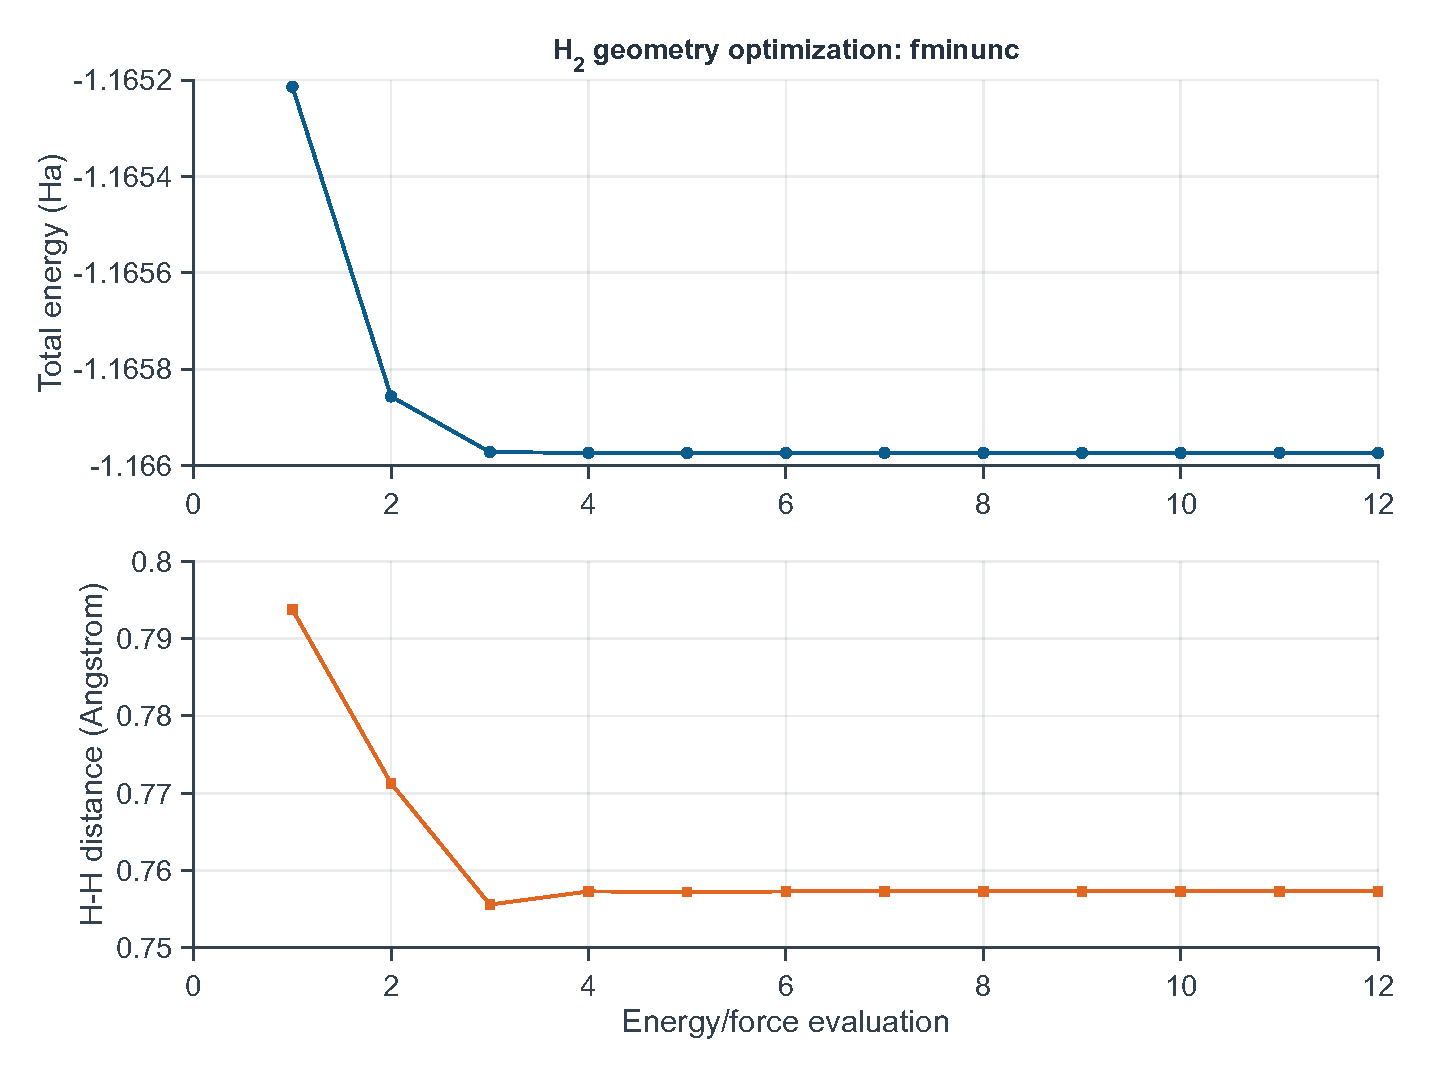
\includegraphics[width=\linewidth]{publication-assets/vector-a7002e532f8546105cf1.pdf}
\caption{氢分子几何优化过程中的能量与键长。横轴为能量与力的函数求值次数，包含优化器的试探构型。}
\label{fig:h2-relax-results}
\end{figure}

函数求值次数、电子迭代次数和几何优化步数不必相同。一些方法需要试探多个位置来寻找合适步长，因此不能把日志中出现的每一个能量值都数成一次被接受的原子移动。

\subsection{本例计算结果}

在所列条件下，fminunc 优化得到的最终键长约为 $1.43107436$ Bohr，即 $0.75729194$ Å。最终总能量约为 $-1.1659737582$ Ha，力范数约为 $5.55\times10^{-5}$ 原子单位，几何优化与最后一次 SCF 均报告收敛。

与初始结构相比，键长略微缩短，能量降低。所得键长对应本例的盒尺寸、泛函、赝势和截断能；改变这些条件后，数值也可能变化。

优化记录保存在工作流结果中，\ui{Structure}中的原始模型保留不变。要在三维查看器中测量最终键长，可导入随书的优化结构\file{examples/h2_optimized.cif}。配套脚本也会保存优化结构，供进一步分析。

\section{对称性分析作为独立工作流}

如果目前只想检查结构的对称性或推荐路径，可以打开二原子原胞示例项目中的 \ui{Symmetry} 模板，而不必先完成一整套电子计算。它适合在导入晶体、建立超胞或施加形变之后，先了解结构是否符合预期。

对称性容差描述允许多大的数值偏差仍把两个位置或晶格参数视为相同。容差过严可能把文件的小量舍入差异识别为降对称，过宽则可能掩盖真实畸变。对于教程提供的理想硅结构，先采用默认设置；对于实验结构或优化后结构，应结合坐标精度解释分析结果。

对称性分析描述几何的空间关系，结构的能量与稳定性则需通过电子结构计算和原子力判断。分析平衡结构时，将对称性结果与优化记录结合阅读。

\section{查看布里渊区}\label{sec:bz-workflow}
\index{Buliyuanqu@布里渊区}

布里渊区图帮助把一维能带路径放回倒空间。能带图中的横轴只表示沿路径行进的距离，无法直接显示路径在多面体中的走向；三维布里渊区图则同时呈现区界、高对称点和路径。这个练习不需要先做SCF。

% Native Online capture, 990 x 660 px after clipping, 254 ppi at 99 mm.
\begin{figure}[H]
\centering
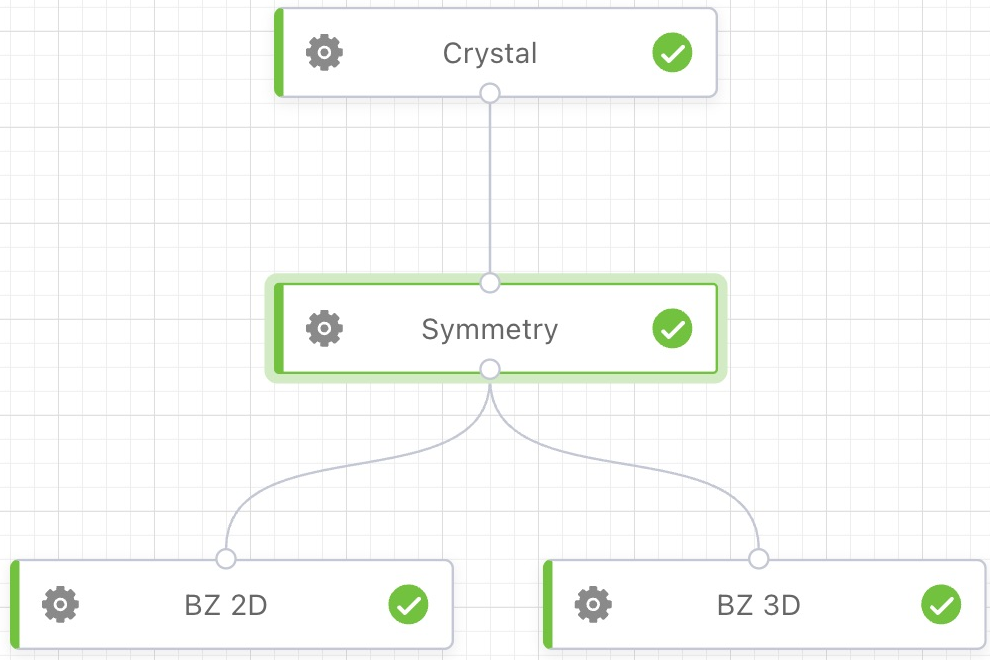
\includegraphics[width=99mm]{publication-assets/crop-7a61cf8df5b1fcc967e4.png}
\caption{\ui{Symmetry}模板的四个节点。\ui{Crystal}将晶体交给\ui{Symmetry}，分析结果分别送往\ui{BZ 2D}与\ui{BZ 3D}。运行完成后，四个节点均显示绿色完成标志。}
\label{fig:si-symmetry-online}
\end{figure}


\begin{steps}
\item 导入\file{silicon_primitive.cif}，在项目的\ui{Structure}中确认出现二位点硅原胞。打开\ui{主页}的\ui{工作流}下拉菜单，选择\ui{从模板建立工作流}\,$\rightarrow$\,\ui{Symmetry}。
\item 模板包含\ui{Crystal}、\ui{Symmetry}、\ui{BZ 2D}和\ui{BZ 3D}四个节点：\ui{Crystal}提供结构，\ui{Symmetry}分析对称性，再分别连接二维与三维图形分支。保留这四个节点，先检查输入。
\item 点击\ui{Crystal}节点的齿轮打开配置，确认任务为\ui{Build Molecule}、类型为\ui{Crystal}，在\ui{Choose imported structures}列表中只选\file{silicon_primitive}。本例保持PBE、\ui{default}赝势、20 Ha、0 K和Nspin=1。这些字段用于建立晶体对象，本流程没有SCF任务。
\item 打开\ui{Symmetry}节点配置，确认任务为\ui{Symmetry \& K-Path}，保持\ui{SymmetryThreshold}为\texttt{1e-7}、\ui{SymmetryPrecision}为\texttt{1e-5}，其余使用默认值。再打开\ui{BZ 3D}节点，确认\ui{Visualization Module}中的任务为\ui{Brillouin Zone 3D}；此节点没有额外专用参数。
\item 保持这份工作流为当前活动文档，点击\ui{主页}\,$\rightarrow$\,\ui{运行}，执行整个流程。两个图形分支都会生成结果，不必先运行SCF，也不必删除\ui{BZ 2D}。
\item 在项目\ui{Results}\,$\rightarrow$\,\ui{Plots}中明确打开\ui{BrillouinZone3D}。如果先显示二维图，从这里切换至三维图。
\item 旋转三维视图，辨认多面体区界、倒格轴以及$\Gamma$、X、U、W、K、L等高对称点，观察路径线在前后表面之间的走向。将点标签及路径段与能带教程中的同一原胞路径对照。
\item 保存项目；在线版使用者再将\file{.ks}项目下载到本机。需要插入报告时，使用结果图工具条的保存入口选择\ui{导出图片}，另存图像，并保存项目。
\end{steps}

% Original Online result export: preserve vector paths and embedded fonts.
\begin{figure}[H]
\centering
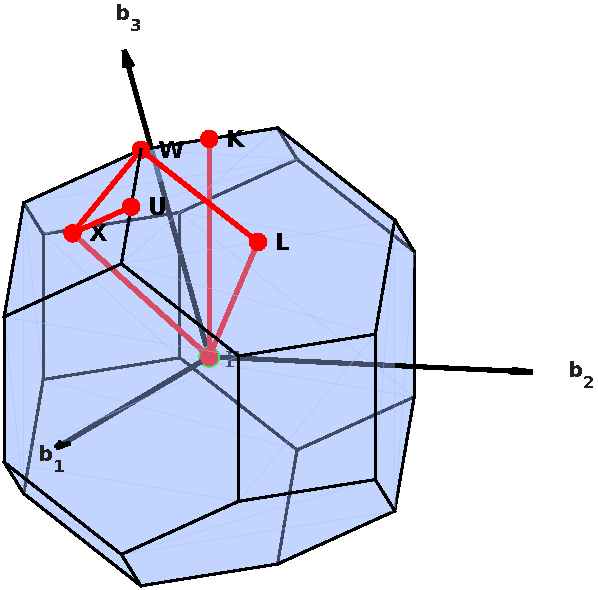
\includegraphics[width=95mm]{publication-assets/vector-cc7185e6fa1fba4c8c34.pdf}
\caption{二位点硅原胞的三维布里渊区。\ui{Symmetry}模板生成的蓝色多面体显示区界，红线连接高对称路径，黑色箭头标明倒格轴。旋转视图可以辨认$\Gamma$、X、U、W、K、L及各段的空间关系；生成布里渊区图无需SCF计算。}
\label{fig:si-bz-online}
\end{figure}


图~\ref{fig:si-bz-online}显示本例的三维布里渊区。随书的\file{Si-primitive-BZ-Online-050.pdf}为矢量图，保留路径线、点标签与倒格轴，适合放大阅读和插入报告。

\ui{BZ 2D}分支的任务为\ui{Brillouin Zone 2D}，按前两个倒格矢的平面信息作图。对于面内倒格矢明确的二维模型，可以另建流程使用这一任务；它不是把任意三维晶体的斜截面自动变成二维材料。因此本节硅原胞以三维图为主要观察对象，练习二维材料时再选用标准放置的二维晶格。两类绘图节点的原胞、路径和对称性选项均在上游配置。

保存后重新打开项目，核对图形、结构与高对称路径，再将需要的视图用于报告。


\section{绘制能带曲面}\label{sec:band-surface}
\index{Nengdai qumian@能带曲面}

路径能带沿若干线段采样；能带曲面则在一张倒空间平面上取点，用曲面高度表示电子能量。它适合观察带边附近的方向变化。这里的“三维”指两个采样坐标加一个能量坐标，不是给整个布里渊区填满三维k点，也不同于第\ref{ch:volume}章的实空间体数据。

先用\file{silicon_primitive.cif}准备一份独立项目，保持晶体类型、PBE、default、20 Ha和原胞SCF网格；把额外能带数设为4，使占据带之外还有空带。小范围练习采用非自旋极化的绝缘体输入，便于辨认最高占据带和最低空带。

\begin{steps}
\item 从SCF流程另存项目，保留\ui{Build Molecule → SCF}两个节点。
\item 在后面依次连接\ui{NSCF}、\ui{Band Calculation 3D}、\ui{Band Structure 3D}。中间节点属于Postprocessing，最后一个属于Visualization。
\item 在NSCF节点保持本书的非自洽选项。打开Band Calculation 3D的选项，按下表填写中心、平面和网格。
\item 保存流程并运行。该流程需要先完成基态求解，再在平面上进行非自洽采样，耗时可能高于只有SCF的流程。
\item 如计算完成，检查Results中出现的\ui{EnergyBandStructure3D}图形。旋转图形观察两张带边曲面，检查它们与采样平面的关系，再保存项目。
\end{steps}

\begin{table}[htbp]
\centering
\caption{能带曲面的小网格配置示例。}
\begin{tabularx}{\linewidth}{lX}
\toprule
选项 & 输入与含义 \\
\midrule
Center KPoint & \literalinput{[0 0 0]}，以Gamma点附近为中心。 \\
Slice Plane & XY；其他选项为XZ、YZ。 \\
Slice Plane Grid & \literalinput{[5 5]}，两个方向各5点，共25个采样点。 \\
Plane Grid Spacing & 0.015，控制当前任务的采样范围；这是倒空间参数，不是原子间距。 \\
\bottomrule
\end{tabularx}
\end{table}

本例每个方向的5个点覆盖中心两侧各0.0375的范围，包含两端点；Plane Grid Spacing在这里控制采样范围。需要严格比较两张曲面时，同时记录中心、平面、点数和范围。

显示任务选取最高占据带与最低空带绘图，能量以本次费米能为零点。两张曲面用于观察带边的色散。图形可能不显示坐标刻度，定量分析时应读取采样数据，并检查网格与范围的收敛。


\section{准备激发态计算}\label{sec:tddft-workflow}
\index{TDDFT@TDDFT}

自洽计算得到基态电子结构。研究电子从基态受到微小扰动后可能出现的激发，需要另一类计算；TDDFT任务提供Casida方法的输入。所需起点是已经收敛的基态电子态，并且必须包含足够的空轨道。只把SCF流程末尾换成TDDFT，却仍只求占据轨道，不能建立所需的激发空间。

\subsection{为氢分子保留空轨道}

以第\ref{ch:first}章同一\file{h2.cif}为起点，另存为独立项目，使用Molecule、PBE、default、20 Ha、Nspin=1。展开Build Molecule高级选项，把\ui{Extra bands}改为4，再运行SCF。这个中性氢分子有一个占据的空间轨道，4条额外带为后续选择空轨道提供输入；它不改变原子数量或总电荷。

在SCF之后添加Computation模块的\ui{TDDFT}节点。选择节点并执行\ui{配置节点}，先查看选项，再展开高级选项。

\begin{table}[htbp]
\centering
\caption{氢分子TDDFT的准备参数。}
\begin{tabularx}{\linewidth}{lX}
\toprule
字段 & 选择与含义 \\
\midrule
TDDFTMethod & casida，当前任务提供的方法。 \\
DiagMethod & direct，直接对角化。 \\
nvbands & 1，选用的占据轨道数。 \\
ncbands & 4，选用的空轨道数；不得超过基态已经求出的额外轨道。 \\
nroots & 3，需要的激发态数，不能超过$nvbands\times ncbands$。 \\
Use TDA & 勾选，使用Tamm--Dancoff近似。 \\
Use IPA / Use RPA & 本例均不勾选；用于另行比较不同响应近似。 \\
\bottomrule
\end{tabularx}
\end{table}

\ui{nvbands}与\ui{ncbands}需要明确填写，本例分别为1和4。TDDFT求解要求Nspin=1。若改变占据轨道数、空轨道数或激发态数，应连同基态额外能带数一起检查。为保留简并的一组跃迁，程序可能增加最终求解的根数；分析时以日志和输出数组中的实际数量为准。

\begin{notebox}{TDDFT求解方式}
图形界面的TDDFT节点存在参数传递问题，不能完成本节的激发态求解。可先按上述设置准备基态与激发空间，再在完整MATLAB\regmark{}中按下一节传入名称/值参数，求得激发能与跃迁向量。相关错误提示为\texttt{Wrong input for tddft\_input}。
\end{notebox}

\subsection{在完整 \headinglatin{MATLAB}\regmark{} 中给出显式参数}

下面代码面向已经初始化KSSOLV数值环境的完整MATLAB\regmark{}，会重新进行含4条额外带的基态计算，再明确传入Casida参数。运行后，可查看基态收敛状态、激发能与跃迁向量。

\noindent\begin{minipage}{\linewidth}
\begin{lstlisting}[language=Matlab]
pseudopotential.PpType('default');
molecule = example.structure.H2();
molecule.ecut = 20;
molecule.funct = 'PBE';
molecule.extranbnd = 4;
scfOptions = options.SCF();
scfOptions.enableGPU = false;
scfOptions.enableParallelPool = false;
[molecule, H, X, scfInfo] = scf(molecule, scfOptions);
if ~scfInfo.converge
    error('Ground-state SCF did not converge.');
end
td = tddft_setup(molecule, scfOptions, H, X, ...
    'method', 'casida', 'diag', 'direct', ...
    'nvbands', 1, 'ncbands', 4, 'nroots', 3, ...
    'istda', true, 'isipa', false, 'isrpa', false);
[excitationHa, transitionVectors] = ...
    tddft_casida_direct(td, molecule);
save('h2-tddft.mat', 'excitationHa', ...
    'transitionVectors', 'scfInfo', 'td');
\end{lstlisting}
\end{minipage}

返回的激发能单位为Ha，换成eV时使用本书的单位换算。跃迁向量描述激发的轨道组合；它不直接等于一条带有展宽和强度的吸收曲线。分析激发时，应结合基态条件、选带数、所用近似与原始结果。


\section{让工作流便于重复和比较}

\subsection{每条流程只承担清楚的任务}

学习时，可以分别保留“硅 SCF”“硅能带”“硅 DOS”三张工作流。这样每张流程的目的都很明确，也更容易检查运行目标。等操作熟练后，再根据需要组合流程或整理为自己的模板。

通过保存并重新导入 \file{.wf} 建立相同工作流后，检查其中的结构选择。原有设置也可能保留原始结构的关联。如果准备计算一个新结构，先改 Build Molecule，再检查相关模型参数。仅修改工作流名称并不会改变计算对象。

\subsection{一个变化配一份说明}

比较参数时，名称可以采用“硅 DOS，4×4×4”和“硅 DOS，8×8×8”这样的简短格式。结果说明中再记录 SCF 网格、额外带数、能量区间和步长。这样既能迅速区分图形，也保留了重现实验所需的信息。

项目里旧图不会因为节点设置改变就自动变成新条件的结果。修改设置后，需要重新运行，并确认新生成的数据与图形属于这次计算。整理项目时可以保留主要比较结果，删除重复或已放弃的试算，让项目仍然容易阅读。

\subsection{完成一条工作流的检查点}

保存后重新打开项目，依次核对结构、节点参数和计算结果，确认运行对象与方法符合说明，结果仍可阅读。对于能带和DOS，还应保留路径或网格以及能量参照。
